\section{Results}
\label{sec:results}

\begin{table*}[t]
  \centering
  \small
  \caption{Chinese paired contrasts on four metrics. Official wF1 and tuple
  accuracy are separate pre-specified Holm families of five. C-wF1 and hF were
  added post hoc; their displayed adjusted values are exploratory and support
  no claim. Intervals are uncorrected 95\% report-cluster bootstrap intervals.}
  \label{tab:contrasts}
  \begin{tabular}{llrrr}
\toprule
Metric & Contrast & $\Delta$ & 95\% CI & $p_{\mathrm{Holm}}$ \\
\midrule
Weighted macro-F1 (official) & M1-M0 & -0.001 & [-0.006, 0.003] & 1.000 \\
 & M3-M2 & -0.001 & [-0.006, 0.004] & 1.000 \\
 & M4-M1 & +0.000 & [-0.005, 0.005] & 1.000 \\
 & M6-M3 & -0.007 & [-0.017, 0.003] & 0.643 \\
 & M6-M5 & -0.009 & [-0.017, -0.001] & 0.135 \\
\midrule
Path-constrained wF1 & M1-M0 & +0.004 & [0.001, 0.007] & \textbf{0.025} \\
 & M3-M2 & -0.001 & [-0.006, 0.004] & 1.000 \\
 & M4-M1 & +0.000 & [-0.005, 0.005] & 1.000 \\
 & M6-M3 & -0.007 & [-0.017, 0.003] & 0.482 \\
 & M6-M5 & -0.009 & [-0.017, -0.001] & 0.108 \\
\midrule
Hierarchical F1 (hF) & M1-M0 & +0.003 & [0.001, 0.005] & \textbf{0.017} \\
 & M3-M2 & +0.002 & [-0.001, 0.005] & 0.302 \\
 & M4-M1 & +0.004 & [0.000, 0.007] & 0.135 \\
 & M6-M3 & +0.006 & [0.000, 0.012] & 0.151 \\
 & M6-M5 & +0.004 & [-0.001, 0.009] & 0.302 \\
\midrule
Tuple accuracy & M1-M0 & +0.035 & [0.028, 0.043] & \textbf{0.001} \\
 & M3-M2 & +0.002 & [-0.003, 0.007] & 0.973 \\
 & M4-M1 & -0.006 & [-0.010, -0.002] & \textbf{0.028} \\
 & M6-M3 & -0.005 & [-0.014, 0.004] & 0.973 \\
 & M6-M5 & -0.004 & [-0.012, 0.004] & 0.973 \\
\bottomrule
\end{tabular}

\end{table*}

\begin{figure*}[t]
  \centering
  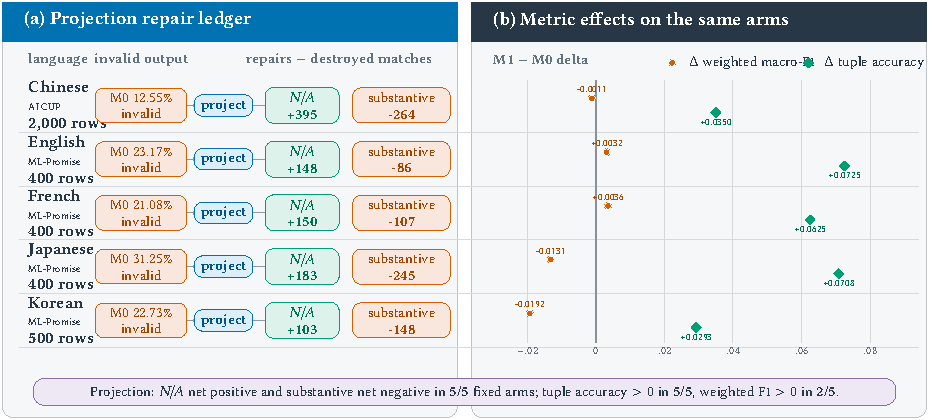
\includegraphics{../figures/figure2_multilingual.pdf}
  \caption{Multilingual projection effects in fixed document-disjoint arms.
  Each row is the preselected $\lambda=0$ M1--M0 arm. Rates and score deltas
  are means over three seeds; repair nets pool the same seeds. Equal-sized
  ledger cards encode signs and exact counts, not comparable magnitudes across
  differently sized corpora. ML-Promise wF1 applies AI CUP weights and is not
  an official ML-Promise metric.}
  \label{fig:multilingual}
\end{figure*}

\paragraph{Chinese confirmatory family.}
Table~\ref{tab:main-results} compares decision rules on identical base
probabilities and Test rows. Independent argmax (M0) produces invalid tuples
for 12.55\% of document-disjoint predictions; projection and 17-state decoding
(M1--M6) reduce this rate to zero by construction. The $\pm$ values are sample
standard deviations across the three seeds. Because each seed determines both
fold assignment and training randomness, they describe spread over the whole
split-and-training pipeline, not a confidence interval.

All five official wF1 contrasts are undetected after Holm correction. For the
central M1--M0 contrast, $\Delta=-0.001$ with 95\% interval
$[-0.006,0.003]$ and $p_{\mathrm{Holm}}=1.000$. This is absence of a detected
difference; it does not establish a zero effect.

\paragraph{Pre-specified tuple family.}
Exact whole-tuple accuracy tells a different story. M1--M0 is $+0.035$
$[0.028,0.043]$, $p_{\mathrm{Holm}}=.001$. Conversely, joint legal-state
decoding is not uniformly better: M4--M1 is $-0.006$
$[-0.010,-0.002]$, $p_{\mathrm{Holm}}=.028$. Searching every legal state can
therefore reduce whole-row correctness relative to greedy projection.

The post-hoc C-wF1 and hF M1--M0 point estimates are also positive
($+0.004$ and $+0.003$), but they do not alter the inferential hierarchy. In
the same-document sensitivity analysis, C-wF1 remains positive at $+0.002$,
while its interval $[-0.001,0.005]$ crosses zero.

\paragraph{Multilingual replication.}
Figure~\ref{fig:multilingual} fixes one arm per language before inspecting
scores. Each uses document-disjoint evaluation and $\lambda=0$.

Across all four external corpora and their four backbones at both loss
settings, M1--M0 tuple accuracy is positive in $32/32$ arms. The weighted
macro-F1 contrast is positive in only $14/32$: English $7/8$, French $5/8$,
Japanese $0/8$, and Korean $2/8$. These are within-arm directions, not a raw
score ranking across languages. For the pre-registered fixed English arm, the
one-sided report-cluster bootstrap tuple effect is $+0.0725$
$[0.0452,0.1019]$ ($p=.0002$; nine report clusters). ML-Promise weighted
scores use AI CUP weights applied to ML-Promise (not official).

\paragraph{Exploratory robustness.}
On the Chinese anchor, training-time structural loss lowers M0 invalidity from
12.55\% to 5.18\%, but its pre-registered M1 wF1 effect is only $+0.00250$
$[-0.00384,0.00860]$ ($p=.427$). Across the 16 external backbone pairs,
structural loss lowers invalidity in $16/16$, while downstream wF1 and tuple
effects are mixed. Chinese DeBERTa and ELECTRA screens likewise reduce
invalidity without a conclusive wF1 gain. Chinese RoBERTa-base emits fewer,
not more, invalid tuples than the large anchor, falsifying the simple
smaller-model mechanism. These screens are descriptive and exploratory.
\FloatBarrier
